\newpage
\section{Nothing but Nets}

In this activity, we are going to build polyhedra out of poster
board. To do this, we're going to draw \textit{nets} of the various
regular polyhedra. The \textbf{net}\index{net of a polyhedron} of a
polyhedron is a single-piece arrangement of polygons that are
connected along their edges so that they can be folded into the
polyhedron. For example, here is the net of a cube:
\[
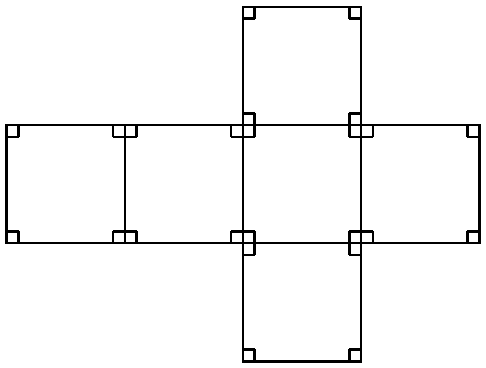
\includegraphics{../graphics/cubeNet.pdf}
\]

\begin{prob}
Sketch another net for the cube. Share your sketch with your
neighbor---does it look OK?
\end{prob}

\begin{prob}
Sketch of a net for a tetrahedron. Share your sketch with your
neighbor---does it look OK? Be sure to label pertinent angles with
their correct measure.
\end{prob}

\begin{prob}
Sketch of a net for an octahedron. Share your sketch with your
neighbor---does it look OK? Be sure to label pertinent angles with
their correct measure.
\end{prob}

\begin{prob}
Sketch of a net for an icosahedron. Share your sketch with your
neighbor---does it look OK? Be sure to label pertinent angles with
their correct measure.
\end{prob}


\begin{prob}
Sketch of a net for a dodecahedron. Share your sketch with your
neighbor---does it look OK? Be sure to label pertinent angles with
their correct measure.
\end{prob}

\begin{prob}
Based on the work from your previous question, construct each of the 5
regular polyhedra. 
\begin{itemize}
\item An edge of your tetrahedron should be $5$ inches in length. 
\item An edge of your octahedron should be $4$ inches in length.
\item An edge of your cube should be $4$ inches in length.
\item An edge of your dodecahedron should be $4$ inches in length.
\item An edge of your icosahedron should be $3$ inches in length.
\end{itemize}
\end{prob}
